The \ac{ahci} is a standard by Intel that defines a common API for \ac{sata}
and SAS host bus adapters. In order to provide backwards-compatibility,
\ac{ahci} specifies modes for both legacy IDE emulation and a standardized
\ac{ahci} interface. 

\ac{ahci} only implements the transport aspect of the communication with
devices. Commands are still transferred as specified in the \ac{ata}/\ac{atapi}
standards.

\section{ATA/ATAPI/SATA}

The \ac{ata} standard specifies an interface for connecting several types of
storage devices, including devices with removable media. \ac{atapi} provides an
extension to allow \ac{ata} to transmit \acs{scsi} commands.

Commands that can be sent to \ac{ata} devices are specified in the \ac{acs}
specifications. Commands in particular interest for this lab project are the
\texttt{IDENTIFY}, \texttt{READ DMA}, \texttt{WRITE DMA} and \texttt{FLUSH
CACHE} commands.

The way these commands are sent to the device is specified in the respective
specification, for example the \ac{sata} or \ac{pata} specifications.

\subsection{SATA}

The \ac{sata} standard specifies the layout of the command \acp{fis} that
encapsulate traditional ATA commands as well as all the lower layers of the
interface to the disk, such as the physical layer.

Figure \ref{fig:h2d_fis} shows the structure of an example \ac{fis}. A Host to
Device Register \ac{fis} can be used to send commands to the disk. The command
value is specified by \ac{ata}. The \ac{fis} contains additional values such as
\ac{lba} and sector count.

\begin{figure}[ht]
\centering
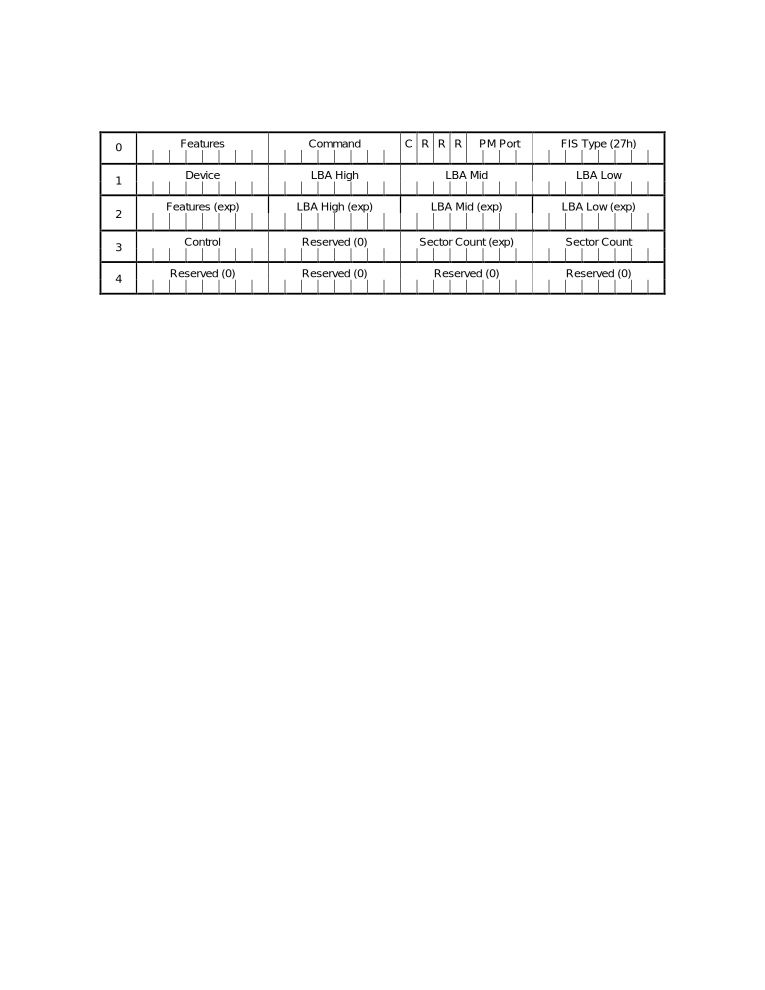
\includegraphics[width=.7\textwidth]{h2d_fis.pdf}
\caption{Host to Device Register FIS \cite[p.~336]{sata_2.6}}
\label{fig:h2d_fis}
\end{figure}

\section{AHCI}

\subsection{Memory Registers}

While the \acs{pci} base address register 0-4 may contain pointers to address
spaces for legacy IDE emulation, \ac{bar} 5 contains the address of the
\ac{hba}'s memory mapped registers. As shown in figure \ref{fig:hba_mem}, this
address space is divided into two areas: global registers for control of the
\ac{hba} and registers for up to 32 ports. A port can be attached to either a
device or a port multiplier. In this lab project, we focus on device handling
and ignore port multipliers.

\begin{figure}[ht]
\centering
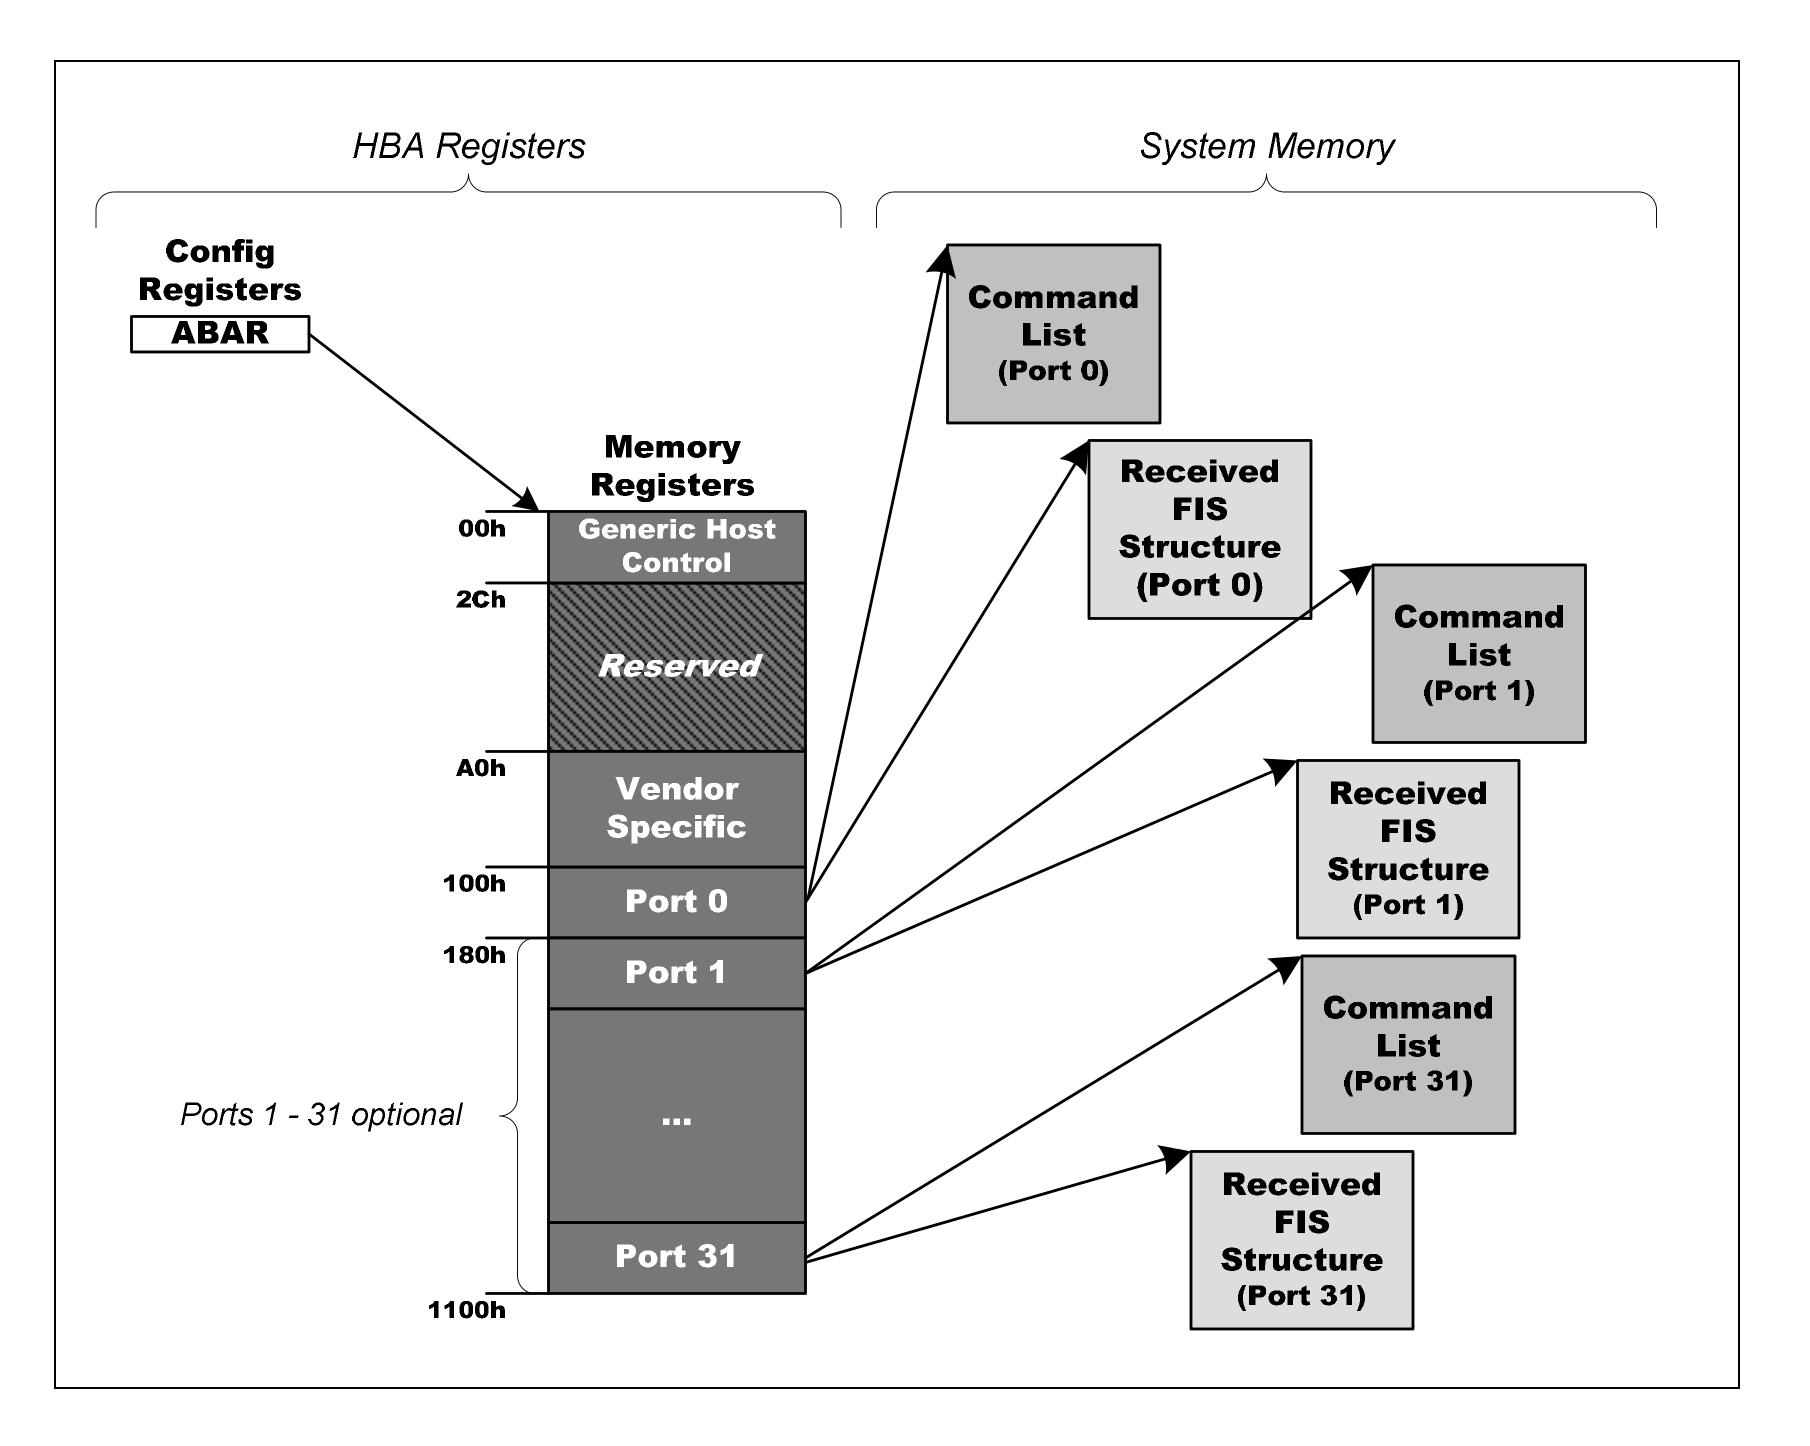
\includegraphics[width=.7\textwidth]{hba_mem.png}
\caption{HBA Memory Space Usage \cite[p.~33]{ahci_1.3}}
\label{fig:hba_mem}
\end{figure}

Every port area (\autoref{fig:port_mem}) contains further control registers and
pointers to the memory regions for the command list and receive \ac{fis} area.
Each of these pointers is a 64-bit value (32-bit for \acp{hba} that don't
support 64-bit addressing) stored in two port registers.

\begin{figure}[ht]
\centering
\includegraphics[width=.9\textwidth]{pmem_overview.pdf}
\caption{Port System Memory Structure adapted from \cite[p.~34]{ahci_1.3}}
\label{fig:port_mem}
\end{figure}

\subsection{Received FIS Area}

The received \ac{fis} area serves as an area where copies of the \acp{fis}
received from the device are stored. The \ac{hba} will copy all incoming
\acp{fis} to the appropriate region of the \ac{rfis} area. If the \ac{hba}
receives an unkown \ac{fis} it is copied to the Unknown \ac{fis} region if it
is at most 64 bytes long. If the \ac{hba} receives an unknown \ac{fis} that is
longer than 64 bytes, it will be considered illegal.

\begin{figure}[ht]
\centering
\includegraphics[width=.8\textwidth]{rfis_area.pdf}
\caption{Received FIS Organization, adapted from \cite[p.~35]{ahci_1.3}}
\label{fig:rfis_mem}
\end{figure}


\subsection{Commands}

A command list (\autoref{fig:command_list}) contains 32 command headers, which
each contain the metadata for a single command.

Commands can be issued to the device by constructing a command header
containing a reference to a command table and further metadata for the command
to be issued.

\begin{figure}[ht]
\centering
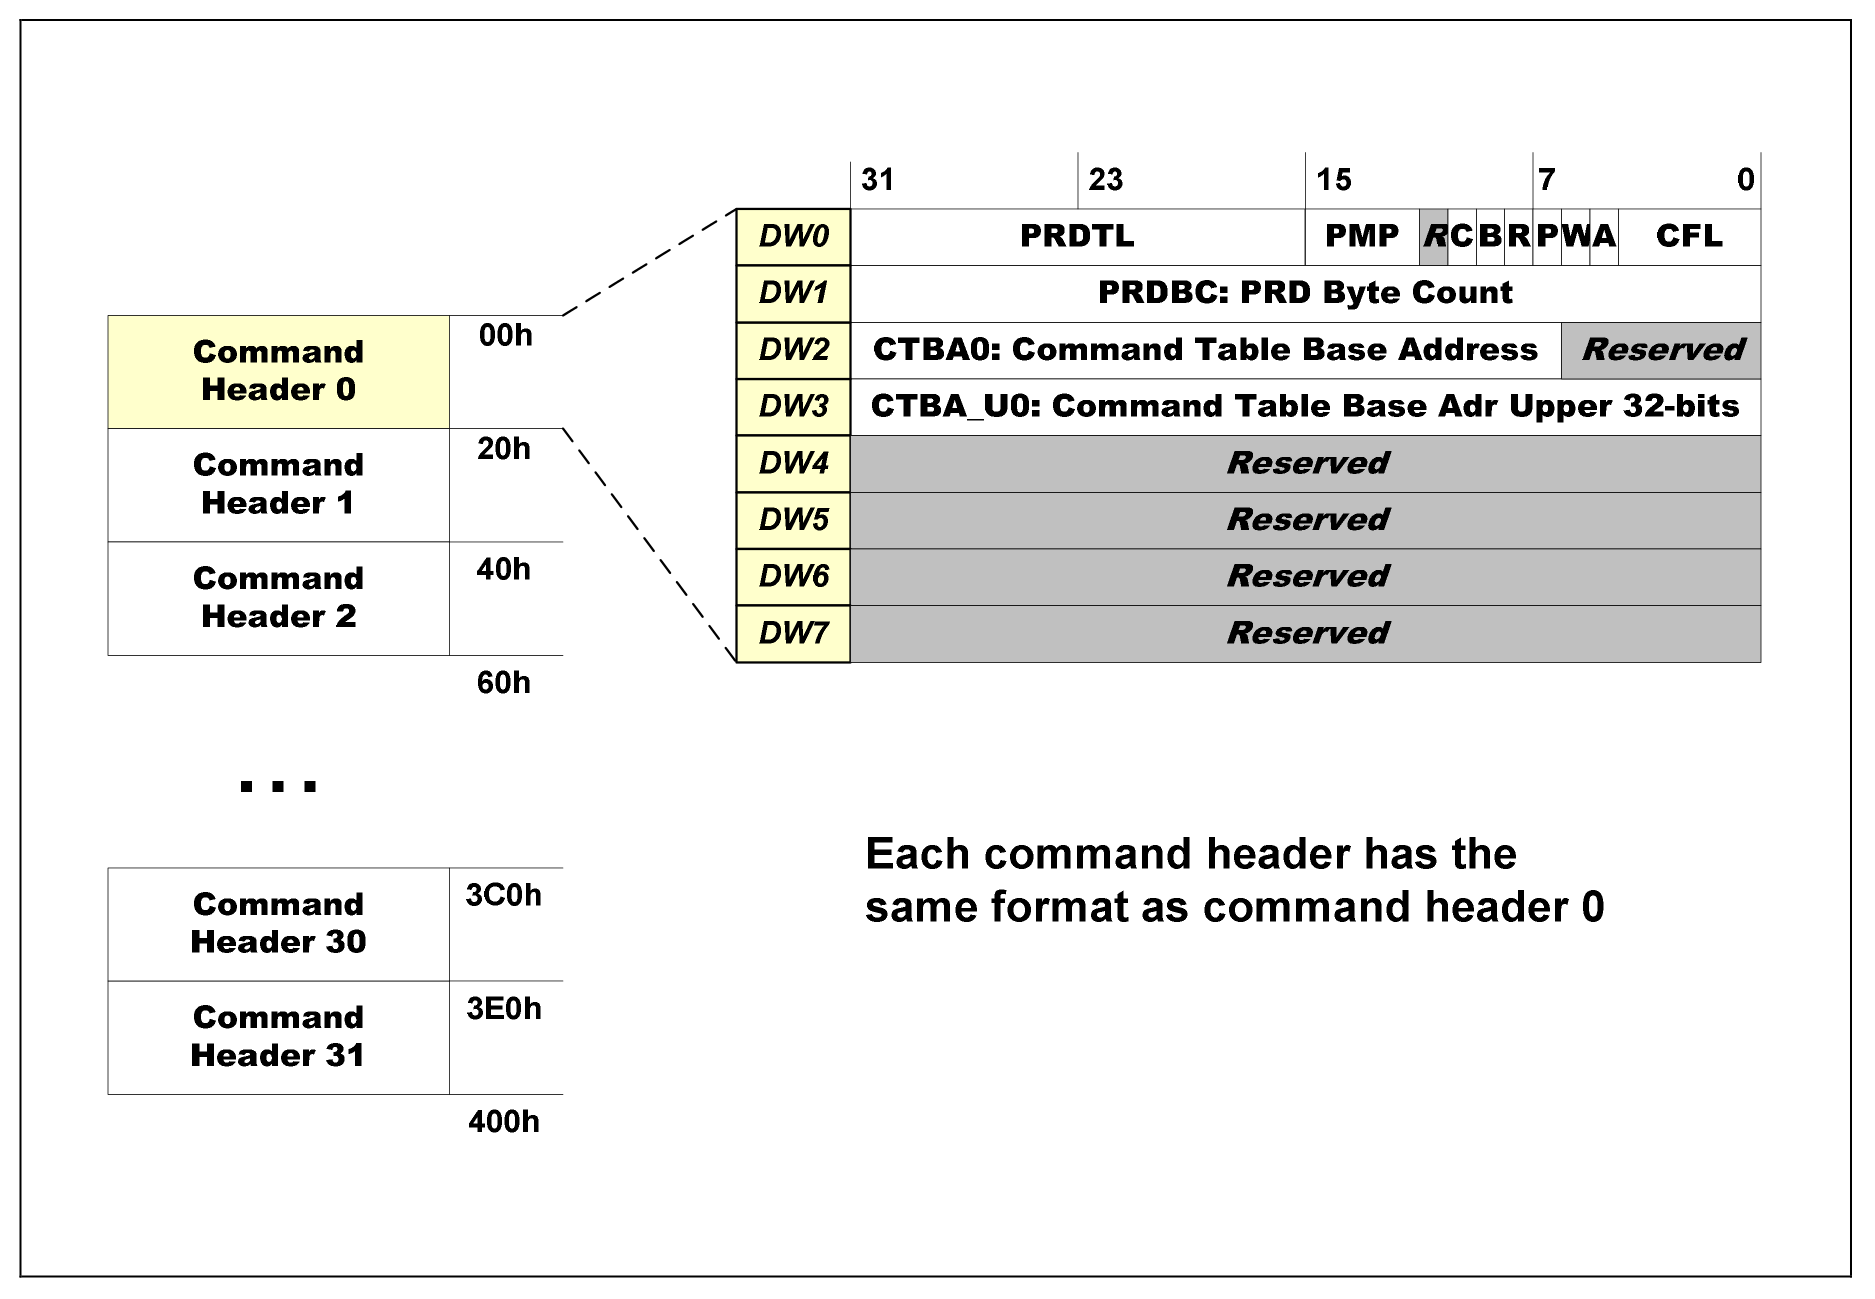
\includegraphics[width=.8\textwidth]{command_list_structure.png}
\caption{Command List Structure \cite[p.~36]{ahci_1.3}}
\label{fig:command_list}
\end{figure}

The command table (\autoref{fig:command_table}) contains the command \ac{fis}
itself and an optional number of physical region descriptors specifying chunks
of main memory in form of a scatter-gather list.

\begin{figure}[ht]
\centering
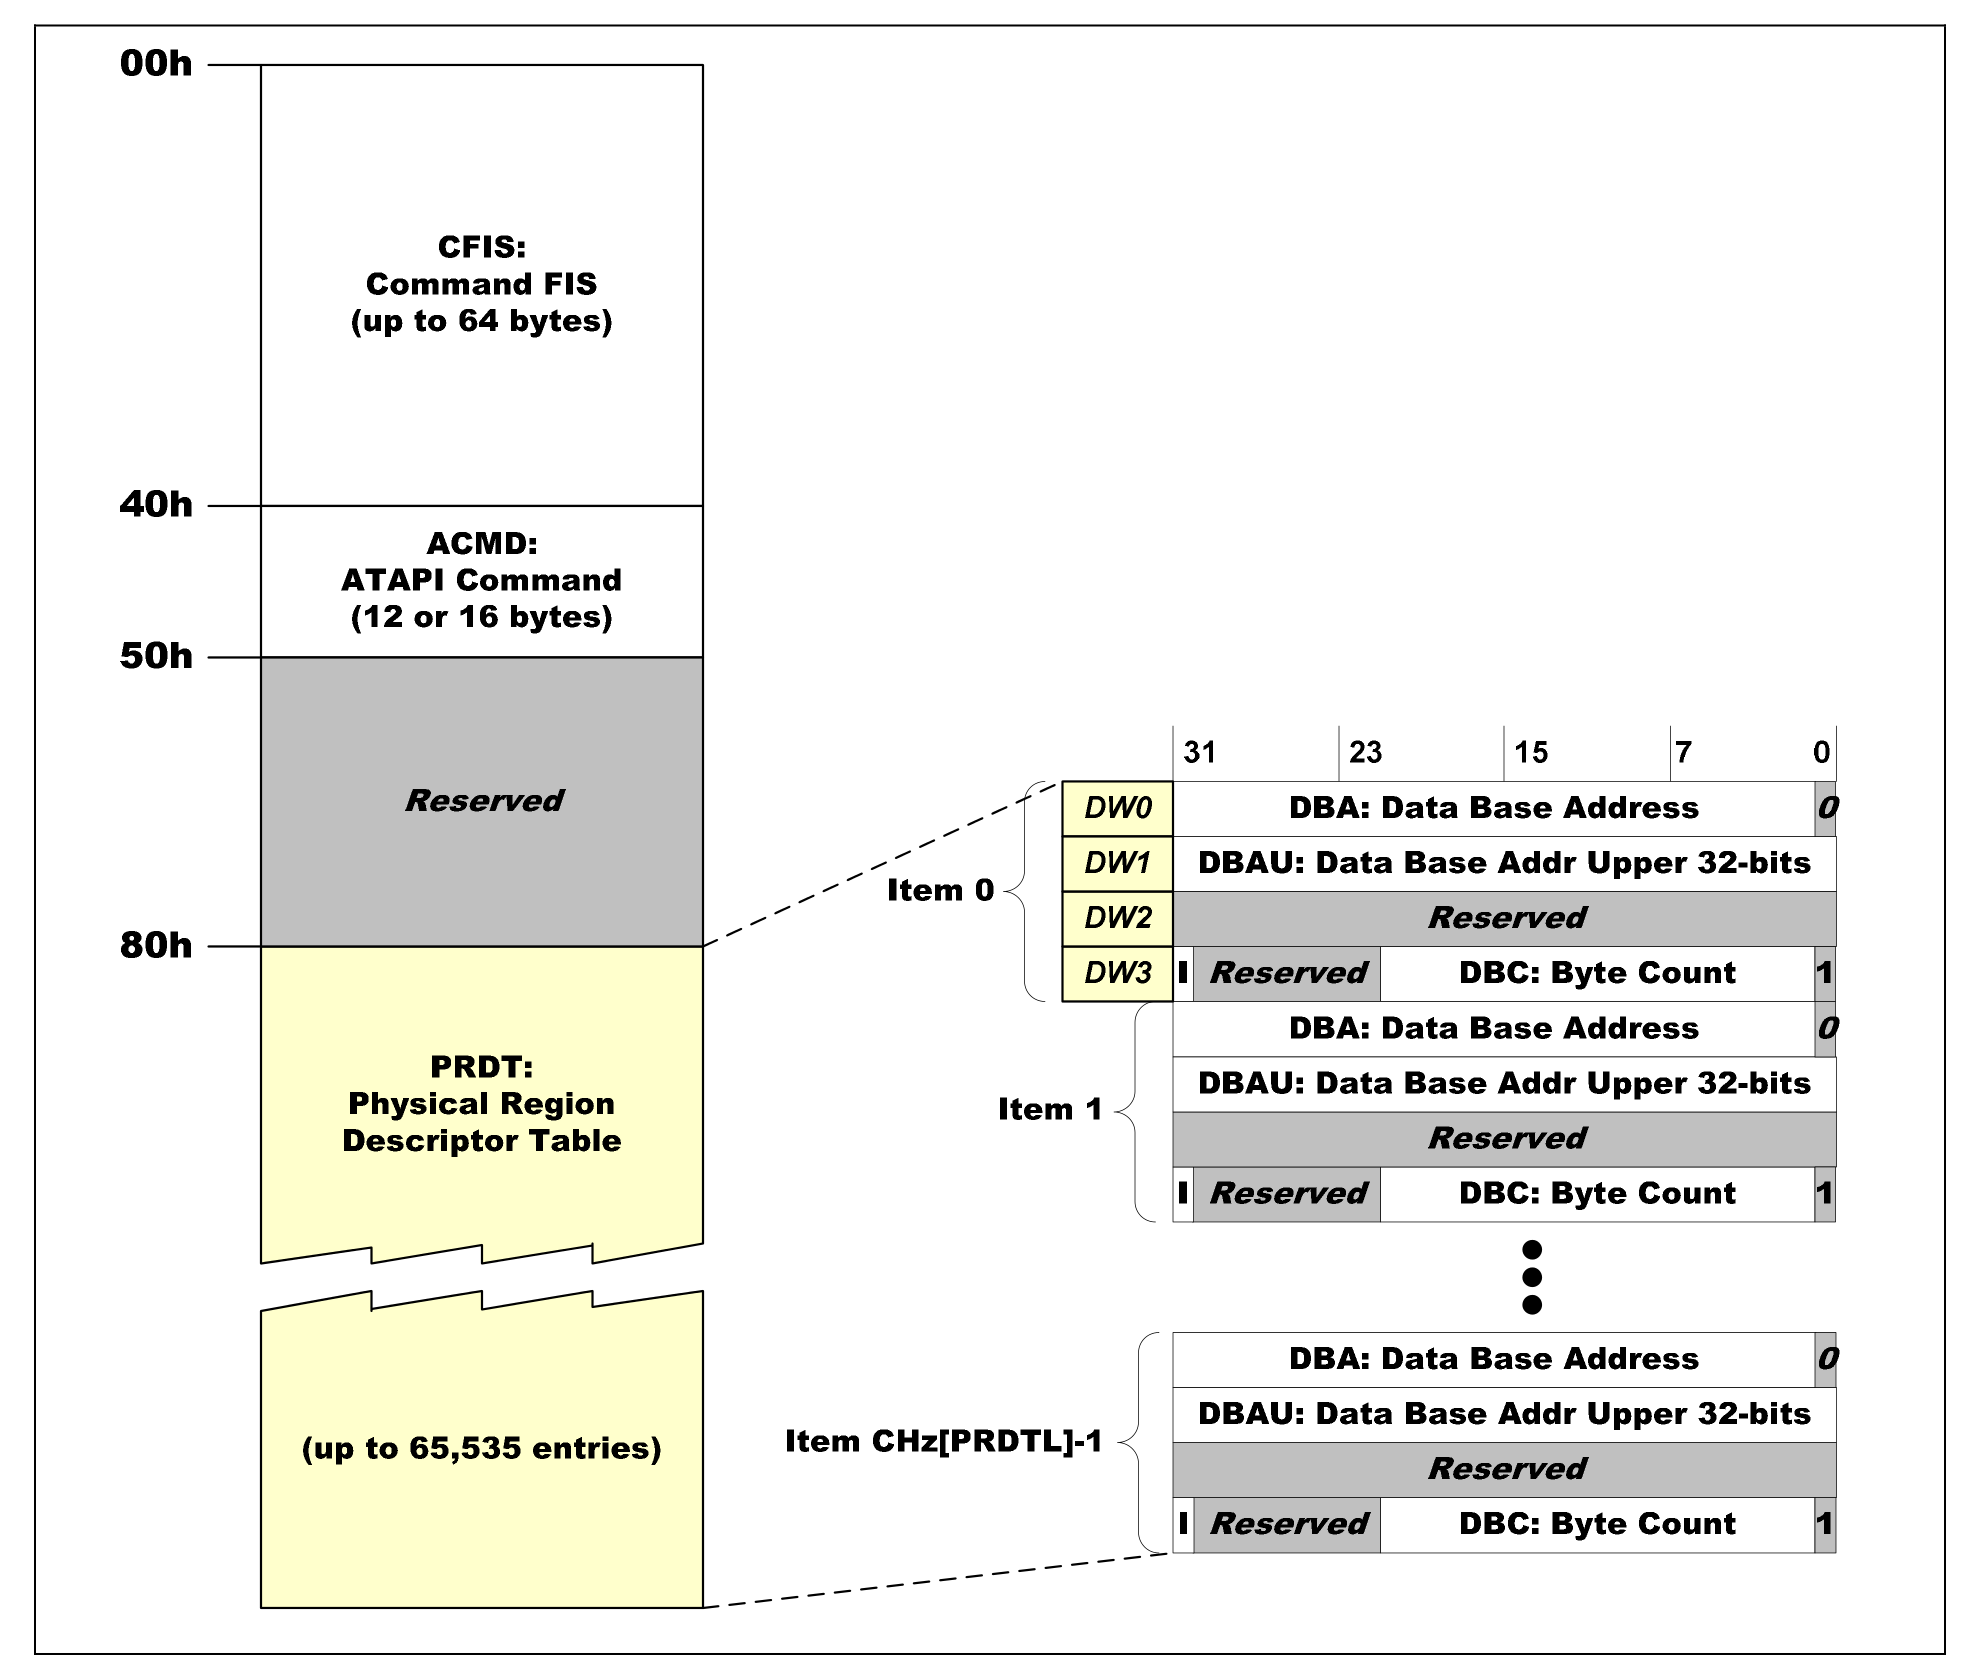
\includegraphics[width=.8\textwidth]{command_table.png}
\caption{Command Table \cite[p.~39]{ahci_1.3}}
\label{fig:command_table}
\end{figure}

Commands are issued by setting the corresponding bit in the command issue
register. Upon command completion, the bit is cleared and if enabled, an
interrupt is triggered.

